% ==========================================================================
%  导言区 · Preamble
% ==========================================================================

\documentclass[11pt, a4paper]{ctexart}

\usepackage{amsmath, amssymb, amsthm, mathtools}
\usepackage{graphicx}
\usepackage{booktabs}
\usepackage{xcolor}
\usepackage{tikz}
\usepackage{geometry}
\usepackage[colorlinks=true, linkcolor=teal, citecolor=teal]{hyperref}
\usepackage{todonotes}
\usepackage{enumitem}
\geometry{margin=2.6cm}

\newtheorem{theorem}{定理}[section]
\newtheorem{lemma}[theorem]{引理}
\newtheorem{proposition}[theorem]{命题}
\theoremstyle{definition}
\newtheorem{definition}[theorem]{定义}
\newtheorem{example}[theorem]{例}

\title{对流扩散方程的谱方法数值分析}
\author{张三 \quad 某某大学数学科学学院}
\date{\today}

\everymath{\displaystyle}
\setlength{\lineskiplimit}{3pt}
\setlength{\lineskip}{5pt}

% ==========================================================================
%  正文 · Document body
% ==========================================================================
\begin{document}
\maketitle

  \begin{abstract}
    \noindent 本文研究一类非定常对流扩散方程的数值求解方法. 我们构造了基于 Legendre 谱离散的高阶格式,
    证明了 $H^1$ 范数下的最优收敛阶, 并通过数值实验验证了理论结果. 研究表明, 该方法在保持谱精度的同时, 对高 Péclet 数问题仍具有良好稳定性.

    \textbf{关键词:} 谱方法; 对流扩散方程; 误差估计; 高精度计算
  \end{abstract}

  \tableofcontents \newpage

  \section{引言}
  \label{sec:intro}

  对流扩散方程广泛应用于流体力学、传热学与化学反应工程等领域\cite{knuth1984tex}. 考虑如下初边值问题: \todo{待补充}

  \begin{equation}
    \label{eq:model}
    \begin{cases}
      \dfrac{\partial u}{\partial t} - \varepsilon \Delta u + \mathbf{b}\cdot\nabla u = f, & (x,t)\in\Omega\times(0,T],\\[4pt] u(x,0) = u_0(x), & x\in\Omega,\\
      u(x,t) = 0, & (x,t)\in\partial\Omega\times[0,T],
    \end{cases}
  \end{equation}
  其中 $\varepsilon>0$ 为扩散系数,$\mathbf{b}$ 为对流速度场. 问题 \eqref{eq:model} 的弱形式可写为:
  \[
  \left( \frac{\partial u}{\partial t}, v \right) + \varepsilon (\nabla u, \nabla v) + (\mathbf{b}\cdot\nabla u, v) = (f, v), \quad \forall v \in H_0^1(\Omega).
  \]

\section{数值格式}
\label{sec:method}

设 $\{\phi_k\}_{k=0}^{N}$ 为 Legendre 基函数，将解展开为
\[
  u_N(x,t) = \sum_{k=0}^{N} \hat{u}_k(t)\,\phi_k(x).
\]
代入问题 \eqref{eq:model} 并取 Galerkin 投影，得到半离散系统
\begin{align}
  \mathbf{M}\frac{\mathrm{d}\hat{\mathbf{u}}}{\mathrm{d}t} + \varepsilon \mathbf{K}\hat{\mathbf{u}} + \mathbf{C}\hat{\mathbf{u}} &= \mathbf{f}(t), \label{eq:semidiscrete}\\
  \hat{\mathbf{u}}(0) &= \hat{\mathbf{u}}_0, \label{eq:ic}
\end{align}
其中 $\mathbf{M}$、$\mathbf{K}$、$\mathbf{C}$ 分别为质量矩阵、刚度矩阵与对流矩阵。

\begin{proposition}
\label{prop:stable}
半离散系统 \eqref{eq:semidiscrete} 在能量范数下是稳定的。
\end{proposition}

\begin{proof}
由 $\mathbf{M}$ 的对称正定性与 $\mathbf{K}$ 的强制性，取测试函数 $v=\hat{\mathbf{u}}$ 可得能量估计。
\end{proof}


  \section{主要结果}
  \label{sec:result}

  \begin{definition}[Sobolev 空间]
    对整数 $m\ge 0$ 与 $1\le p<\infty$, 定义
    \[
    W^{m,p}(\Omega) = \left\{ v\in L^p(\Omega): D^{\alpha}v \in L^p(\Omega),\ |\alpha|\le m \right\}.
    \]
  \end{definition}

  \begin{lemma}[Poincaré 不等式]
    \label{lem:poincare}
    存在常数 $C>0$, 使得对任意 $v\in H_0^1(\Omega)$ 有 $\|v\|_{L^2}\le C\|\nabla v\|_{L^2}$.
  \end{lemma}

  \begin{theorem}[最优收敛阶]
    \label{thm:main}
    设 $u\in H^{s}(\Omega)$,$s\ge 1$,$u_N$ 为谱 Galerkin 解. 则存在与 $N$ 无关的常数 $C>0$ 使得
    \[
    \|u-u_N\|_{H^1} \le C N^{1-s}\|u\|_{H^s}.
    \]
  \end{theorem}

  \begin{proof}
    由投影算子的逼近性质与双线性形式的强制性可得, 详见文献~\cite{lamport1994latex}.
    \begin{example}
      取 $\varepsilon=10^{-3}$,$\mathbf{b}=(1,1)^{\mathsf{T}}$, 此时 Péclet 数约为 $10^{3}$, 属于对流占优问题.
    \end{example}
  \end{proof}

  \section{数值实验}\todo{待补充}\todo{待补充}
  \label{sec:numerics}

  表~\ref{tab:error} 给出了不同网格规模下的 $L^2$ 误差与收敛阶, 结果与定理~\ref{thm:main} 的预测一致.

  \begin{table}[htbp]
    \centering
    \caption{不同网格规模下的误差与收敛阶}
    \label{tab:error}
    \begin{tabular}{lccc}
      \toprule $N$ & $L^2$ 误差 & 收敛阶 & 耗时 (ms) \\
      \midrule 16 & $3.21\times 10^{-3}$ & -- & 12 \\
      32 & $8.02\times 10^{-4}$ & 2.00 & 31 \\
      64 & $2.01\times 10^{-4}$ & 2.00 & 96 \\
      \bottomrule
    \end{tabular}
  \end{table}

  \begin{figure}[htbp]
    \centering 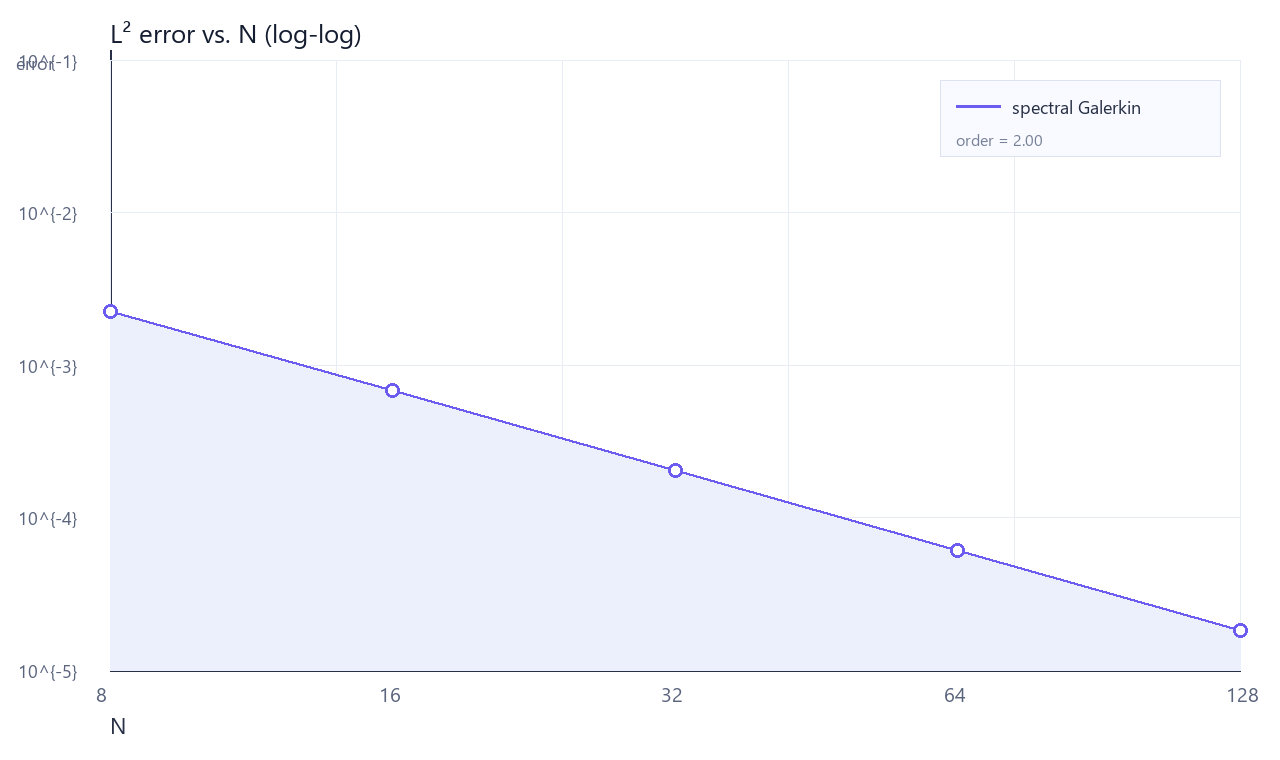
\includegraphics[width=0.72\linewidth]{figures/spectrum.png}
    \caption{不同网格规模下的 $L^2$ 误差收敛曲线}
    \label{fig:compare}
  \end{figure}

  \begin{figure}[htbp]
    \centering
    \begin{tikzpicture}[scale=0.85, >=stealth]
      \draw[->] (0,0) -- (6.2,0) node[right] {$x$}; \draw[->] (0,0) -- (0,3.4) node[above] {$u$}; \draw[thick, teal, domain=0:5.6, samples=120] plot (\x, {2.6*exp(-0.55*\x)}); \draw[thick, dashed, orange, domain=0:5.6, samples=120] plot (\x, {2.6*exp(-0.55*\x)*(1+0.35*sin(deg(3*\x)))}); \node[teal, right] at (4.3,0.55) {精确解}; \node[orange, right] at (4.3,1.55) {数值解 $u_N$};
    \end{tikzpicture}
    \caption{TikZ 示意图: 一维衰减解与数值解的对比}
    \label{fig:tikz}
  \end{figure}

  如 图~\ref{fig:compare} 与 图~\ref{fig:tikz} 所示, 数值解在整个区域上与精确解高度吻合.

  \section{结论}
  \label{sec:conclusion}

  本文给出了对流扩散方程谱 Galerkin 格式的最优误差估计, 并通过数值实验加以验证. 后续工作将考虑自适应时间步长与并行实现.
  \begin{equation}
    a^2=1
  \end{equation}
  \begin{enumerate}[label=(\chinese*)]
    \item 1
  \end{enumerate}
\bibliographystyle{plain}
\bibliography{references}

\end{document}
